%%%%%%%%%%%%%%%%%%%%%%%%%%%%%%%%%%%%%%%%%
% Short Sectioned Assignment
% LaTeX Template
% Version 1.0 (5/5/12)
%
% This template has been downloaded from:
% http://www.LaTeXTemplates.com
%
% Original author:
% Frits Wenneker (http://www.howtotex.com)
%
% License:
% CC BY-NC-SA 3.0 (http://creativecommons.org/licenses/by-nc-sa/3.0/)
%
%%%%%%%%%%%%%%%%%%%%%%%%%%%%%%%%%%%%%%%%%

%----------------------------------------------------------------------------------------
%	PACKAGES AND OTHER DOCUMENT CONFIGURATIONS
%----------------------------------------------------------------------------------------

\documentclass[paper=a4, fontsize=11pt]{scrartcl} % A4 paper and 11pt font size

\usepackage[T1]{fontenc} % Use 8-bit encoding that has 256 glyphs
\usepackage{fourier} % Use the Adobe Utopia font for the document - comment this line to return to the LaTeX default
\usepackage[english]{babel} % English language/hyphenation
\usepackage{amsmath,amsfonts,amsthm} % Math packages

\usepackage{graphicx}

\usepackage{sectsty} % Allows customizing section commands
\allsectionsfont{\centering \normalfont\scshape} % Make all sections centered, the default font and small caps

\usepackage{fancyhdr} % Custom headers and footers
\pagestyle{fancyplain} % Makes all pages in the document conform to the custom headers and footers
\fancyhead{} % No page header - if you want one, create it in the same way as the footers below
\fancyfoot[L]{} % Empty left footer
\fancyfoot[C]{} % Empty center footer
\fancyfoot[R]{\thepage} % Page numbering for right footer
\renewcommand{\headrulewidth}{0pt} % Remove header underlines
\renewcommand{\footrulewidth}{0pt} % Remove footer underlines
\setlength{\headheight}{13.6pt} % Customize the height of the header

\numberwithin{equation}{section} % Number equations within sections (i.e. 1.1, 1.2, 2.1, 2.2 instead of 1, 2, 3, 4)
\numberwithin{figure}{section} % Number figures within sections (i.e. 1.1, 1.2, 2.1, 2.2 instead of 1, 2, 3, 4)
\numberwithin{table}{section} % Number tables within sections (i.e. 1.1, 1.2, 2.1, 2.2 instead of 1, 2, 3, 4)

\setlength\parindent{0pt} % Removes all indentation from paragraphs - comment this line for an assignment with lots of text

%----------------------------------------------------------------------------------------
%	TITLE SECTION
%----------------------------------------------------------------------------------------

\newcommand{\horrule}[1]{\rule{\linewidth}{#1}} % Create horizontal rule command with 1 argument of height

\title{	
\normalfont \normalsize 
\textsc{BRSU} \\ [25pt] % Your university, school and/or department name(s)
\horrule{0.5pt} \\[0.4cm] % Thin top horizontal rule
\huge Neural Networks\\Assignment 3 \\ % The assignment title
\horrule{2pt} \\[0.5cm] % Thick bottom horizontal rule
}

\author{Bastian Lang} % Your name

\date{\normalsize\today} % Today's date or a custom date

\begin{document}

\maketitle % Print the title

\section{Read chapter 2 from Haykin's book (2nd edition), till the section 2.6 inclusive and then start from 2.10 till 2.12 inclusive. Summarise or sketch your insights in mind-map or an outline or a summary.}

See figure \ref{fig1}.

\begin{figure}[ht]
	\centering
  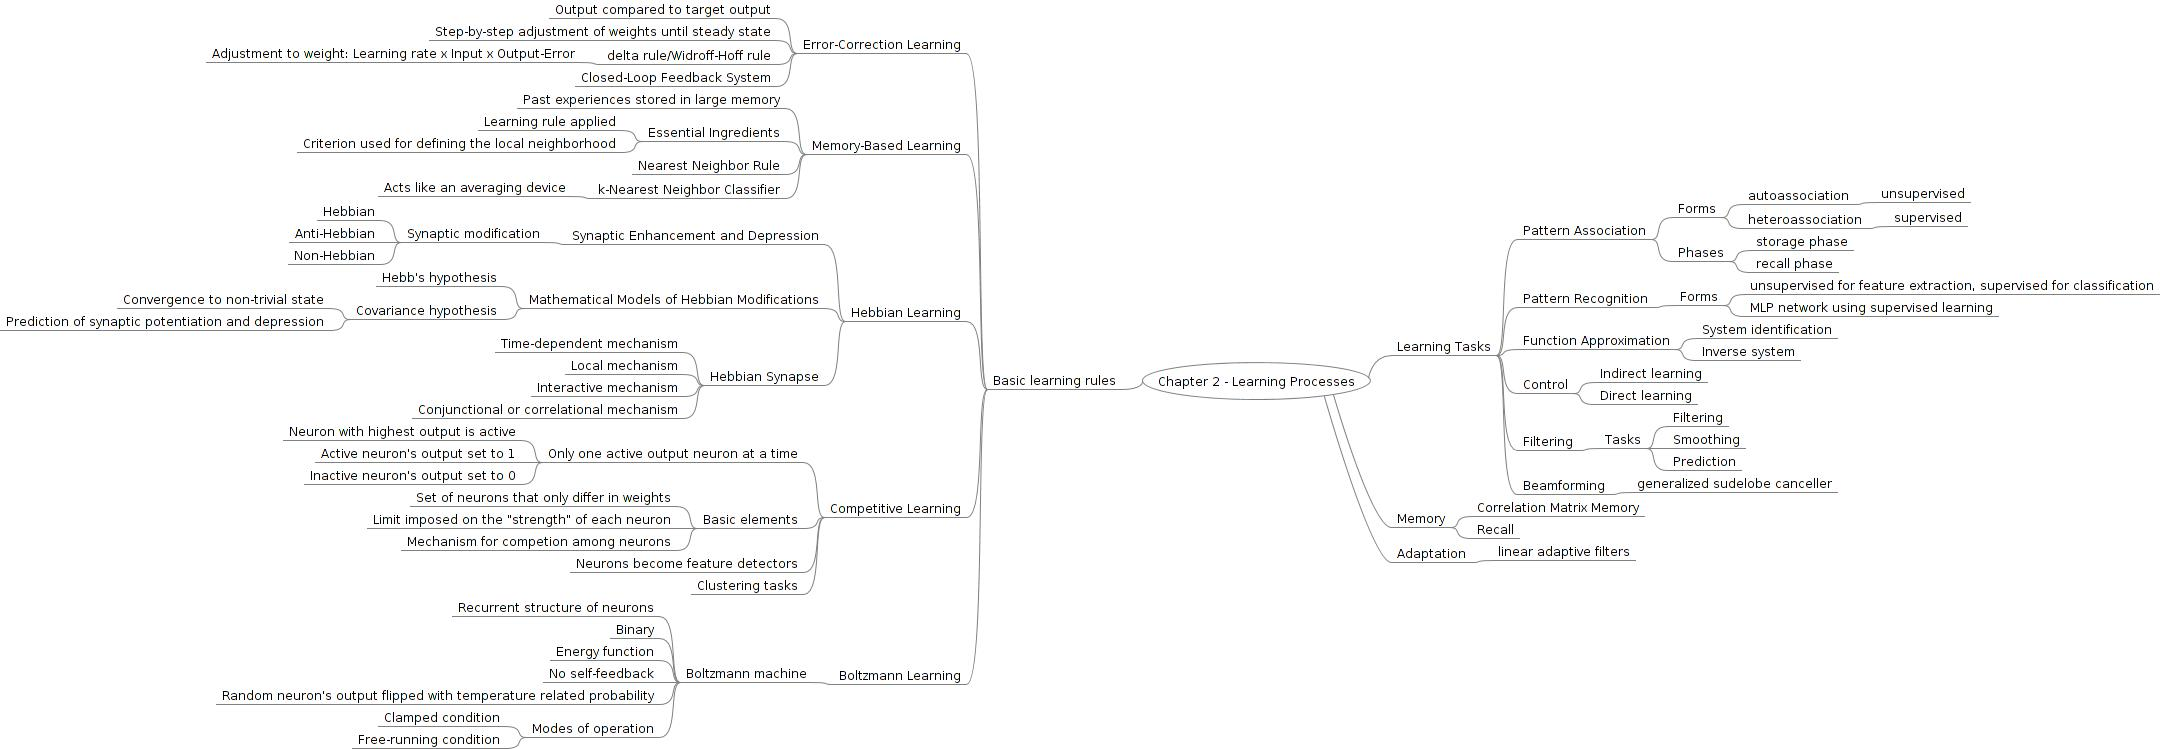
\includegraphics[width=1\textheight, angle=90]{mindmap.jpeg}
	\caption{Mindmap}
	\label{fig1}
\end{figure}

\section{From the Chapter 2 Haykin's book solve 2.1}

The \textit{delta rule} is a supervised learning method. It uses a teacher to compute the error of the network output and uses this error to adjust the neuron's weights.\\\\

The \textit{Hebb's rule} is a form of unsupervised learning. The weights of synchronously active neurons get strengthened, the weights of asynchronously active neurons get weakened or eliminated.

\section{From the Chapter 2 Haykin's book solve 2.10}

$y_i = \phi (v_i)$\\
$v_i = \sum_{j}^{N}{x_jw_{ij}} - \sum_{k\neq i}^{M}y_kz^{-1}c_{ki}$\\
with N the number of input neurons and M the number of output neurons.\\
The neuron with the largest value for v is considered active and its output equals 1, all the other outputs are set to 0.

\section{From the Chapter 2 Haykin's book solve 2.21}

\section{A simple network is given below (from lecture slides). You have to update the weights once using Boltzmann learning for this network. Please do calculations by hand or by using MATLAB or Python.}

\end{document}